\chapter{Project Context}
\section*{Introduction}
\addcontentsline{toc}{section}{Introduction}
\par This chapter introduces the foundational context for the development of \mbox{VitamiNurse}, a nutritional mobile application created during my internship at ONRTECH. 

Our goal is to develop a personalized recommendation system and an AI assistant for nutritional guidance. The system presents product details, assesses the scanned product with AI, and then provides a clear conclusion regarding the compatibility with the user’s nutritional profile.
The chapter also explains the basic theories behind the project , compares existing nutrition applications to show their limitations, and presents VitamiNurse as an innovative solution. Finally, we justify the use of the Scrumban methodology for team management and the CRISP-DM framework for technical development.

\section{Presentation of the host company}
\par ONRTECH\footnote{\url{https://onrtech.fr/}} is a French company, operating since 2020 and located in
Villiers-sur-Marne, France, that focuses on software development, IT consulting, and artificial intelligence.
It operates within the wider field of programming, advisory, and other digital services, delivering modern, innovative solutions tailored to evolving business needs. 
\par Since its creation, ONRTech has rapidly grown into a trusted provider of digital services, having collaborated with numerous
clients throughout France and Europe. More than just a tech provider, it positions itself as a durable digital partner by focusing on customer satisfaction and offering customized solutions.
\begin{figure}[H]
    \centering
    
\includegraphics[width=0.25\textwidth]{images/ONRTECH_logo.jpeg}
    \caption{ONRTECH company logo}
    \label{fig:onrtech_logo}
\end{figure}


\newpage
\section{Internship context and project objectives}
As part of our training at the Higher Institute of Computer Science and Mathematics in Monastir, we had the opportunity to complete our end-of-studies internship at ONRTECH.

 The goal of this internship is to develop a personalized recommendation system and an AI assistant for the nutritional mobile app Vitaminurse. The system presents product details, assesses the scanned product with AI, and then shows a clear conclusion of the analysis on whether the product is suitable for the user’s nutritional profile. If it is not suitable, the recommendation system suggests more adapted alternatives.

In addition, it engages users in friendly conversation and provides personalized nutritional advice. By understanding the preferences, health goals, and nutritional needs of each person, Vitaminurse provides personalized advice and recommendations that actually make sense for their lifestyle and health needs. 
\subsection{First version of VitamiNurse}
The initial version of VitamiNurse exists as a simple mobile application developed by ORTECH  to enable users scan product barcodes for viewing nutritional data. The application operates in a market which presents major obstacles to its success because of intense competition. The food tracking market already has two established apps Yuka and OpenFoodFacts which makes it difficult for VitamiNurse to get noticed. The app does not have special features that would help it stand out from other apps. The entire user interface operates with lower interactivity than top competitors, which results in decreased user involvement and reduced user retention. The study of current food monitoring applications together with their performance details will help identify user requirements for this domain.

\begin{center}
\begin{figure}[ht]
            \centering
            
\includegraphics[scale=0.55]{images/VN_app_logo.png}
            \caption{VN app logo} 
            \label{fig:VN app logo}
        \end{figure}
\end{center}

\section{Problem Statement and Challenges}

The increasing focus on healthier lifestyles has driven demand for tools that support informed dietary choices. However, many individuals struggle to navigate the complexities of nutrition due to limitations in existing mobile applications. These tools often fail to provide personalized, reliable, and practical guidance, leaving users without the support they need to make balanced food choices. This section presents an analytical review of various applications in the field of food monitoring in order to reformulate a clear vision of an more advanced version of \mbox{VitamiN-urse}. 

\par The study is based on both the examination of relevant references and the comparative analysis of competing applications currently available in the market.

\subsection{Analysis of Key Competitor Applications}
To understand the competitive landscape and identify areas for improvement, we analyzed several leading nutritional applications: Yuka, Open
Food Facts, QuelProduit, and Food Check. Each of these apps offers
unique features but also exhibits significant limitations that our proposed
solution aims to address.

\subsection{Yuka}
With over 74,000 users, Yuka\footnote{\url{https://yuka.io/}} is a widely used nutritional mobile application, particularly in France and the United States. As shown in Figure \ref{fig:yuka_evaluation}, it scans food and cosmetic products to provide a quick quality rating:
excellent, good, mediocre, or bad.
\begin{center}
\begin{figure}[H]
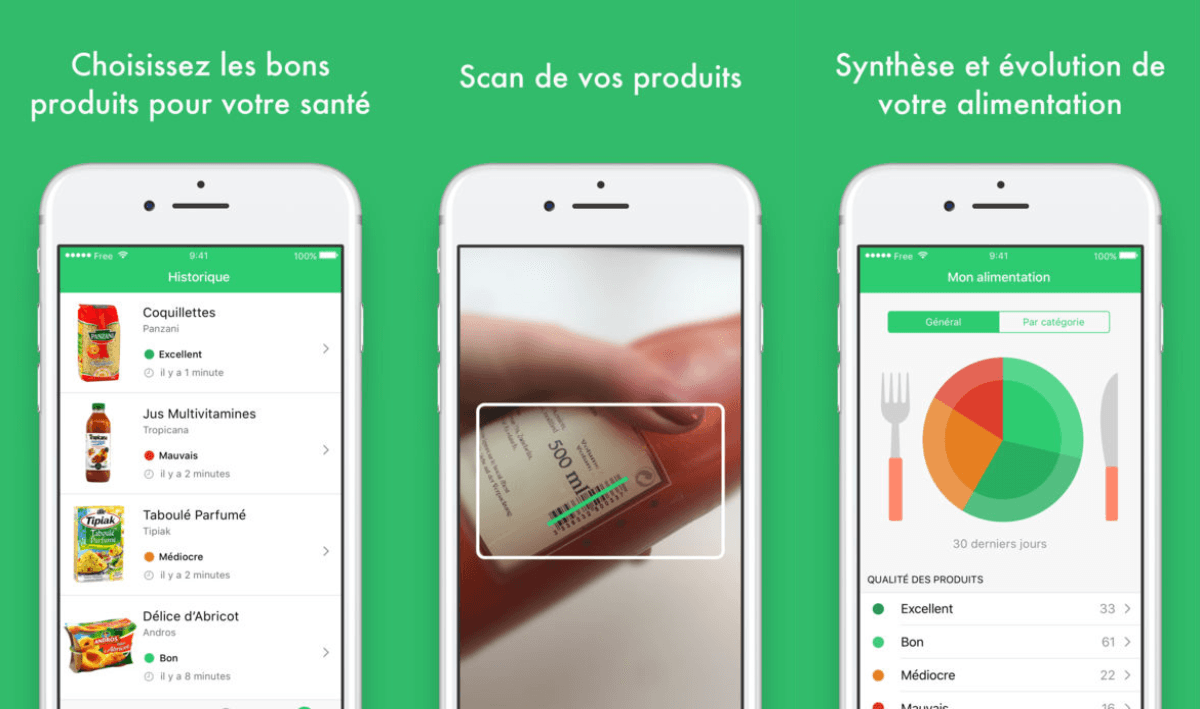
\includegraphics[scale=0.35]{images/yuka_evaluation.png}
\caption{The Yuka system for product evaluation}
\label{fig:yuka_evaluation}
\end{figure}
\end{center}
\par Its intuitive interface and simple scoring system based on composition,
additives, and organic status help users make quick purchasing decisions.
Despite these advantages, Yuka also presents notable limitations. Its
database is not always updated regularly. In addition, the application
lacks personalization by overlooking individual dietary goals, allergies,
and health conditions. As a result, Yuka serves more as a tool for initial
screening than as a source of personalized nutritional guidance.
\subsection{ Open Food Facts}
Open Food Facts\footnote{\url{https://fr.openfoodfacts.org/}} is a collaborative and nonprofit database of food
products. It is the primary data source for many other applications,including Yuka. It is true that the Open Food Facts application provides transparent
information such as ingredients, allergens, and Nutriscore. But Open Food Facts suffers
from significant usability challenges. The lack of personal tracking or goal
setting features limits its usefulness for consumers seeking a nutritional
guide.
% OFF 00-01-02-03
\begin{figure}[H]
    \centering
    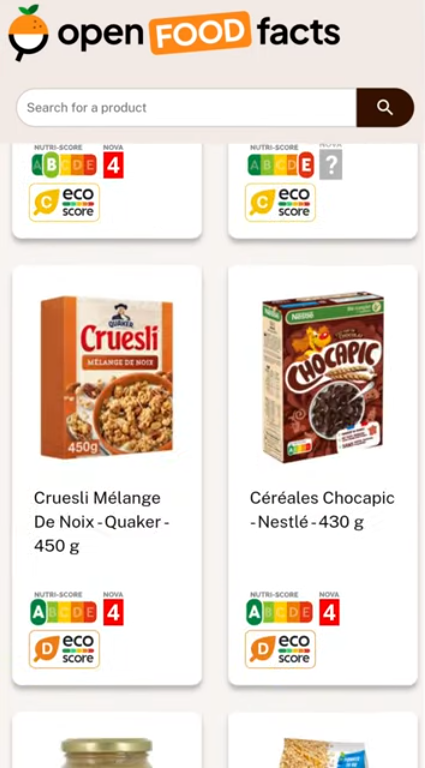
\includegraphics[width=0.24\textwidth]{images/OFF-00.png}
    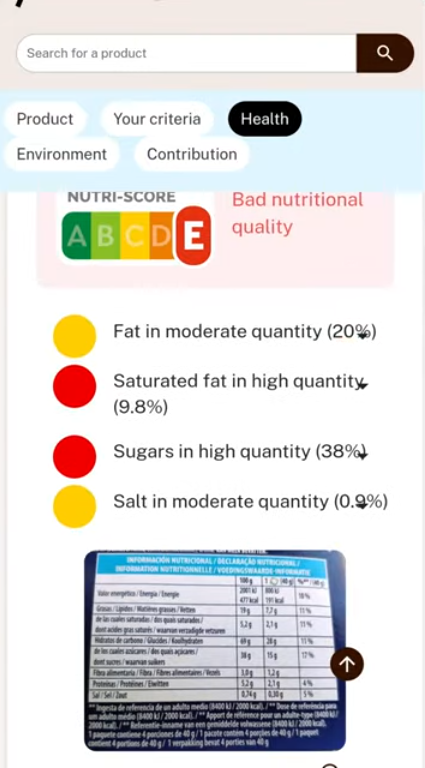
\includegraphics[width=0.24\textwidth]{images/OFF-01.png}
    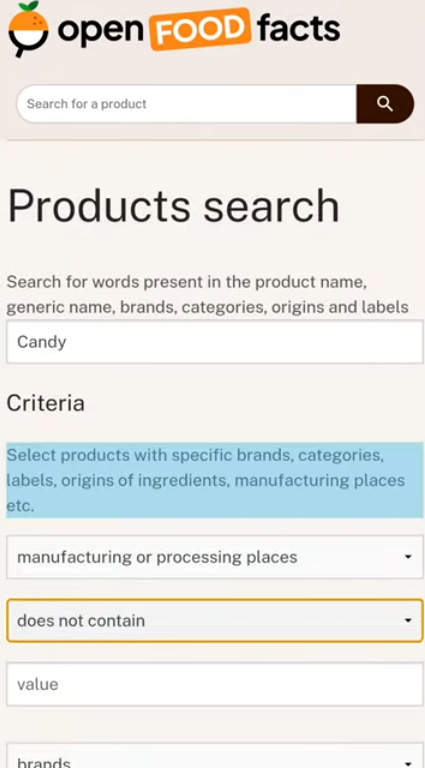
\includegraphics[width=0.24\textwidth]{images/OFF-02.png}
    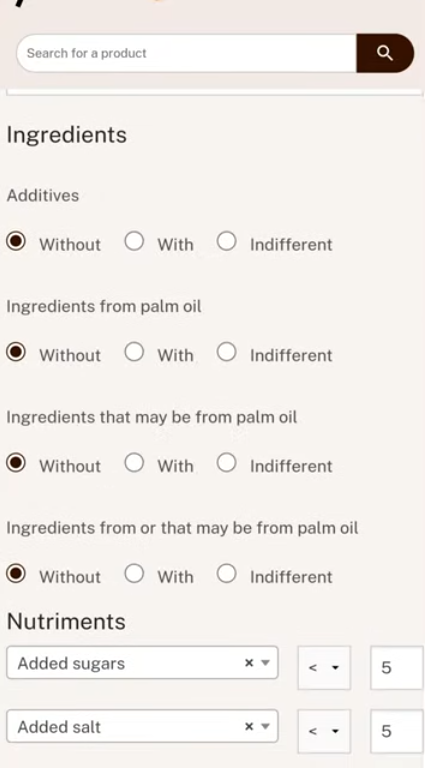
\includegraphics[width=0.24\textwidth]{images/OFF-03.png}
    \caption{Lack of personalization and user-friendly features in the OFF app}
    \label{fig:natilait_screenshots}
\end{figure}

\subsection{QuelProduit}
\par QuelProduit\footnote{\url{https://www.quechoisir.org/application-mobile-quelproduit-n84731/}} is a product 
analysis app developed by the French non-profit consumer organization \textbf{UFC-Que Choisir} \footnote{\url{https://www.quechoisir.org/}}, to help users make
safer choices by scanning barcodes to evaluate food, cosmetic, and house-
hold items. 

 \begin{center}
\begin{figure}[H]
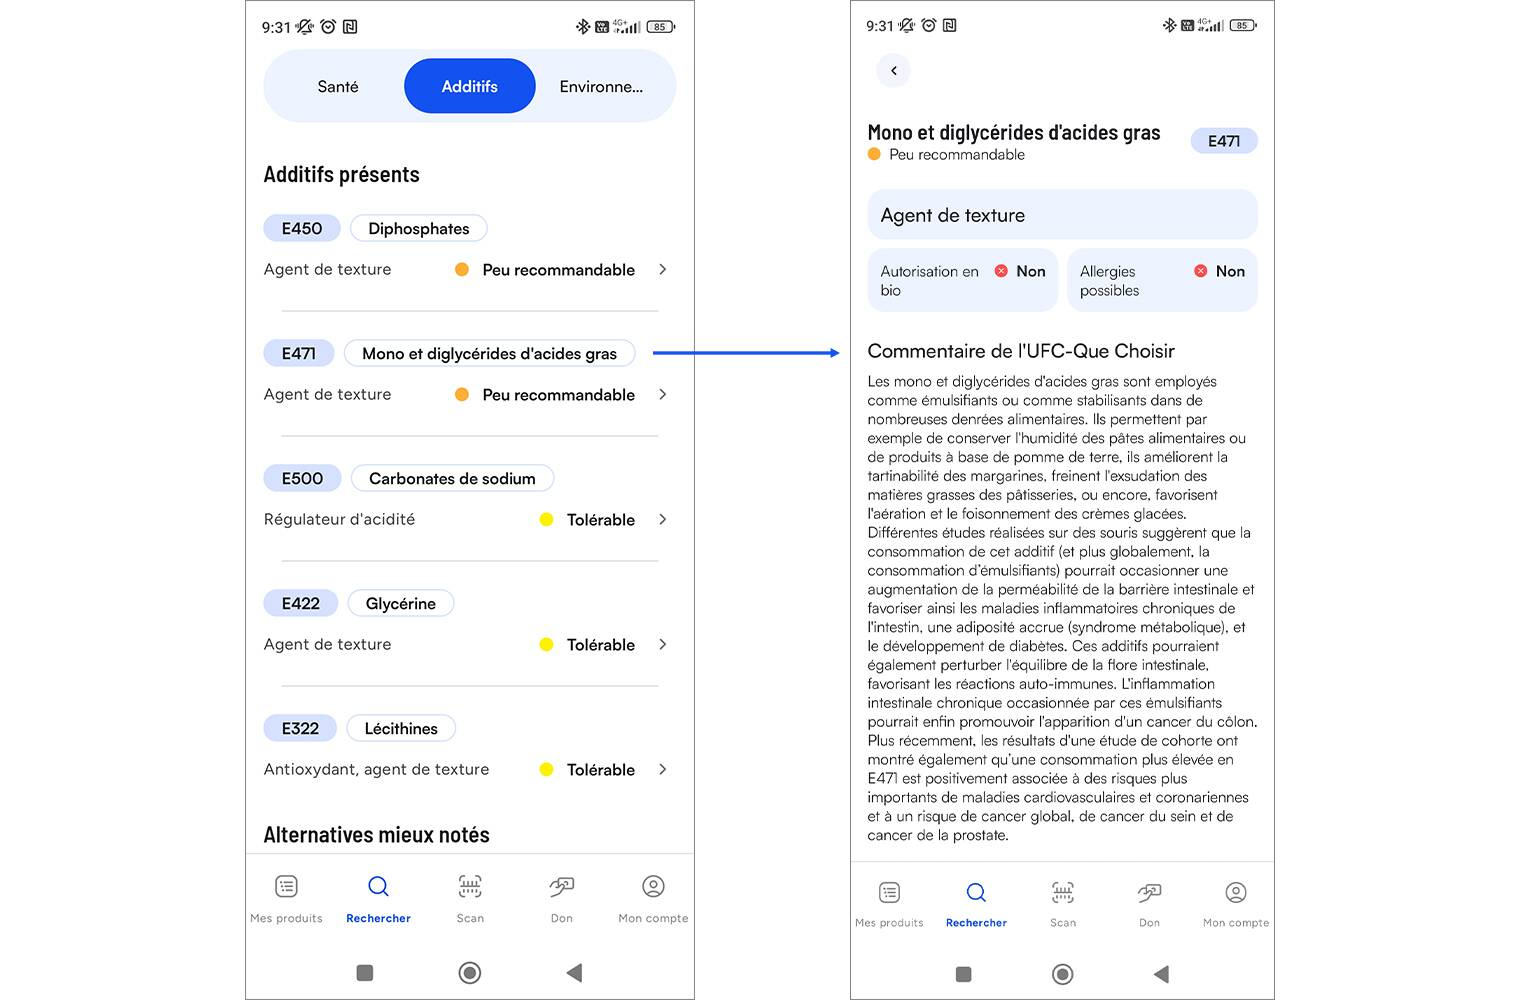
\includegraphics[scale=0.19]{images/quelproduit.jpg}
\caption{Identification of harmful substances and food additives by the QuelProduit application}
\label{fig:queChoisir}
\end{figure}
\end{center}

\par The application focuses on consumer safety by highlighting
harmful substances, but does not offer balanced nutritional guidance or
personalized dietary support. Users should view this tool as a simple
detection system rather than a nutritional guide or assistant.


\subsection{Food Check}
Food Check\footnote{\url{https://play.google.com/store/apps/details?id=com.bytes_and_pixels.food_buddy&hl=fr}} is an AI-powered nutritional scanner application developed by 
Bytes \& Pixels \footnote{\url{https://www.bytes-and-pixels.de/}}. The application offers AI chatbot assistance and personalized recommendations.

\begin{figure}[H]
\centering
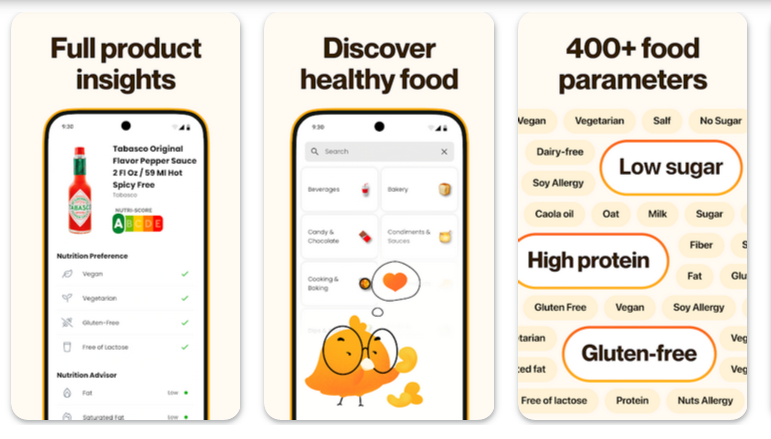
\includegraphics[scale=0.45]{images/food_check.png}
\caption{The complexity of parameters required from the user in the scanner application Food}
\label{fig:foofCheck}
\end{figure}

The main problem is the complexity of parameters to enter by user
to receive personalized recommendations. The onboarding process is
described as intrusive, requiring extensive personal information before
delivering value. This complexity can deter users from fully engaging
with the app, as illustrated in Figure

\subsection{Key Challenges and gaps in Current Applications}

There are a number of significant deficiencies of current nutritional apps.
The table\ref{tab:competitor_evaluation} summarizes the evaluation of key competitor applications
based on several criteria: frequency of database updates, recommendation
system sophistication, presence of a chatbot, level of user interaction,
and depth of product evaluation. This analysis highlights the strengths
and weaknesses of each application, providing a clear framework for
identifying opportunities to enhance VitamiNurse. Existing nutrition
applications frequently fall to deliver a comprehensive user experience.
Many provide basic recommendations by simple category-based filtering
that do not account for individual factors such as allergies and medical
conditions. This lack of personalization can make it difficult for users
to find relevant and actionable advice. Furthermore, the widespread
use of simplified scoring systems further reduces complex nutritional
data to a single value, which can mislead users and prevent informed
decision-making.
In the first three applications, there is a lack of interactivity. Real-time
chatbot guidance is missing to answer questions and provide tailored recommendations and advice. The lack of conversational guidance restricts
the ability of apps to provide dynamic and context-aware support.
For Food Check, this application does not consider user health conditions
evolution. The app requires users to input detailed personal information
during onboarding. This approach fails to adapt to changes in health status or dietary goals automatically over time, limiting long-term relevance
and effectiveness of recommendations.
% in Figure \ref{fig:yuka_feedback}. 

\begin{table}[htbp]
\centering
\small % Reduces font size to \small (you can also use \footnotesize for even smaller)
\caption{Evaluation of Key Competitor Applications}
\label{tab:competitor_evaluation}
\begin{tabularx}{1.15\textwidth}{|l|X|X|X|X|}
\hline
\textbf{Feature} & \textbf{Yuka} & \textbf{Open Food Facts} & \textbf{QuelProduit} & \textbf{Food Check} \\
\hline
Database Frequency Update & Not Frequent & Varies (by users) & Moderate & Moderate \\
\hline
Recommendation System & Elementary & Basic & Basic & Elementary \\
\hline
Chatbot & Absent & Absent & Absent & Present \\
\hline
Interaction & High & Moderate & Moderate & Moderate \\
\hline
Product Evaluation & Comprehensive & Comprehensive & Detailed & Detailed \\
\hline
\end{tabularx}
\end{table}


 
\section{Proposed solution}
  
To address the identified market gaps, we propose a comprehensive
enhancement of the VitamiNurse application. Our vision is to transform it from a simple product scanner into an intelligent, adaptive, and
indispensable nutritional partner. This transformation is centered on delivering a uniquely personalized and interactive user experience through
the following key features.

\begin{figure}[H]
\centering
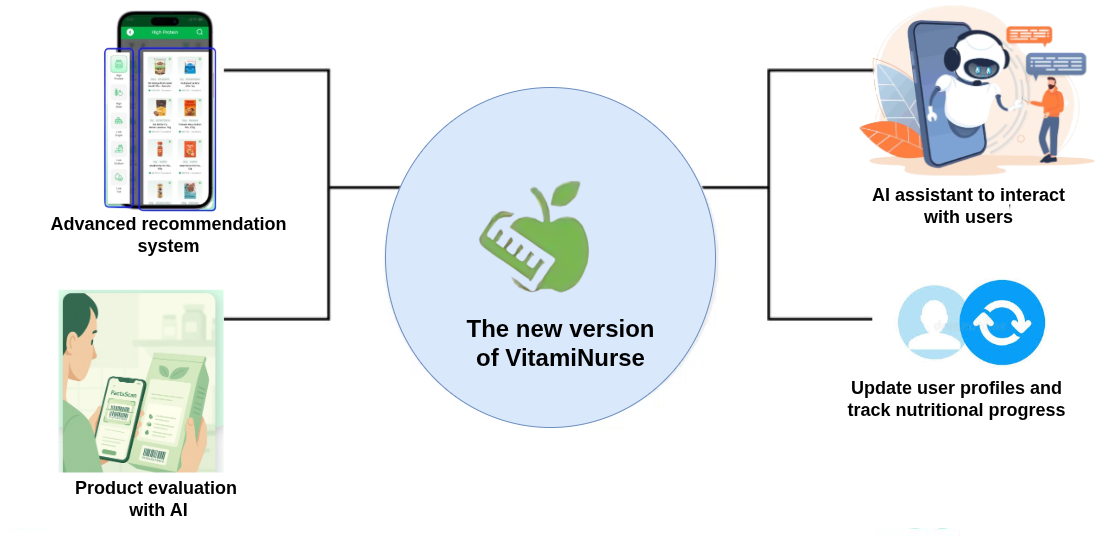
\includegraphics[scale=0.45]{images/new_version_VN.png}
\caption{Features of the new version of VitamiNurse}
\label{fig:VN_new_features}
\end{figure}

\subsection{An Interactive Nutritional Assistant}

To bridge the interactivity gap found in competing applications, VitamiNurse will feature a friendly AI assistant integrated directly into the
user experience.
\par This 24/7 assistant serves as a conversational partner
for all nutritional inquiries, providing dynamic support that goes beyond
simple question–answer chatbots.
The assistant will be capable of answering a wide range of questions,
from clarifying nutritional information to offering meal suggestions based
on preferences and dietary restrictions of each user.

\subsection{Personalized Product Recommendations}
We recognize that nutritional needs are highly individual. Moving beyond
generic scoring systems, VitamiNurse will provide deeply personalized
guidance. The application learns from user preferences, dietary restrictions, and health goals to offer tailored product recommendations.
For example, if a user is managing hypertension, the app will prioritize low-sodium options when suggesting alternatives to scanned products. 
This level of personalization ensures that users receive relevant and actionable advice that aligns with their unique health profiles.

\subsection{Product Evaluation Using AI}

The application functions as a personal nutritionist at the point of sale.
It transcends simply listing ingredients by performing a sophisticated
evaluation tailored to the user’s unique health profile, whether it be for
weight management, diabetes, or hypertension.


\subsection{Continuous Updates of Product Database and User Profiles}

A fundamental limitation of existing applications is the lack of current
and accurate product information. Our solution ensures that users can
have complete confidence in the data they access. The system is designed
to automatically and continuously refresh its database by using a data
pipeline from trusted sources.
Without the need for manual updates, the application will maintain
dynamic user profiles in real-time that evolve with the user’s health
status and dietary goals. This adaptability ensures that recommendations
remain relevant over time, accommodating changes in lifestyle, health
conditions, and personal preferences. By continuously updating both
product data and user profiles, VitamiNurse aims to provide a truly
personalized and trustworthy nutritional guidance experience.


\section{Project Methodology}

The first step to ensure the smooth running and success of any project
is choosing the right methodology. Today,Scrum, XP, and Kanban and
Scrumban are the most popular agile approaches in web and mobile
development. To choose the best approach, we decided to compare and
select the one that best fits our context and objectives.

\subsection{Comparative Study of existing methodologies}
\subsubsection{a) Scrum Method} 
Scrum is an agile methodology that promotes collaboration, adaptability, and the iterative delivery of high-quality results. This method encourages agile teams to meet regularly to review project progress and adjust their direction as needed. This dynamic approach balances investment and the final product, ensuring greater customer satisfaction and optimal value delivery \cite{scrum2025}.
The main elements of Scrum are:

\begin{enumerate}[label=\textbf{-}]
    \item \texttt{Sprint:} Is a working cycle with fixed duration, of one to four weeks. In this case, it is the Scrum Master to ensure that this period is not exceeded \cite{schwaber2004agile}

    \item \texttt{Scrum Master:} Their main role is to facilitate the application of Scrum principles and resolve blockages.

    \item \texttt{Scrum Team:} A multidisciplinary, self-organizing team that manages the planning and delivery of features.


    \item \texttt{Product Owner:} He validates the functionalities, prioritizes the requirements and user expectations.

    
\end{enumerate}
\subsubsection{b) Kanban Method}
Kanban, originating from Japanese industry, is a visual workflow management tool. It allows you to visualize and limit work in progress in software development and IT work . The main elements of Kanban are as follows:

Kanban, originating from Japanese industry, is a visual workflow management tool. It allows you to visualize and limit work in progress in software development and IT work\cite{anderson2010kanban}. The main elements of Kanban are as follows:A \texttt{Kanban board} visualizes workflow steps ("To do", "In progress", "Done"), \texttt{Kanban cards} represent tasks with their details (description, deadlines), and \texttt{WIP} (Work In Progress) reduces overloads and quickly identifies bottlenecks.

\subsubsection{c) XP Method (eXtreme Programming)}

XP takes agile principles to the extreme with rapid iterations and enhanced customer collaboration with minimal documentation. It is characterized by frequent code reviews and a creative and collaborative working environment through pair programming\cite{beck2000extreme}. 


By performing frequent code reviews and unit tests to make changes quickly, it seeks the best quality and customer satisfaction that remains in constant contact throughout the project. This approach is based on 5 values: \texttt{Simplicity}, which is favored by the search for easier solutions to achieve objectives; \texttt{communication} in direct communication between team members on the one hand and the client on the other; \texttt{feedback} through the constant exchange of feedback between the project team and key customers; \texttt{courage} required to undertake changes such as exploring new paths; and \texttt{respect} for each team member and their work.


\subsubsection{d) Scrumban Method}
Scrumban is a hybrid methodology that combines the flexibility of Kanban board with the rigor of Scrum sprints. Scrum roles are incorporated while enabling real-time modifications and the best possible workflow visualization. The team does, in fact, follow certain rituals, use sprints, and assign roles to the Scrum Master and Product Owner. Nonetheless, the procedure is less exacting than Scrum, enabling teams to maintain an ideal workflow and make real-time priority adjustments.

\begin{center}
\begin{figure}[H]
            \centering
            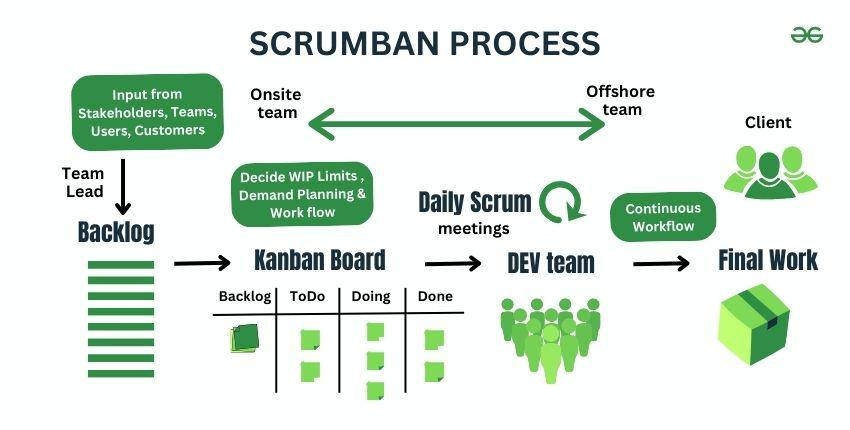
\includegraphics[scale=0.44]{images/scrumban.jpg}
            \caption{Scrumban Process }
            \label{fig:Scrumban_Process}
\end{figure}
\end{center}   


\subsection{Chosen Team Management Methodology: Scrumban}
Our selection of the Scrumban methodology is based on an analysis of the limitations of pure approaches (Scrum, XP, Kanban) in the practical plan in the host company as well as the specific needs of our project. Generally, we can summarize the identified problems as follows:
\begin{itemize}
    \item \textbf{Limited numbers:}
    The XP (eXtreme Programming) approach requires development pairs (pair programming), which is difficult to apply with the available human resources.
        
    \item \textbf{Accelerated Scrum Pace:}
    Short sprints (2–4 weeks) can generate excessive pressure on the development team, risking compromising quality, especially for an end-of-study internship.    
        
    \item \textbf{Flexibility needs:}
    The rigidity of Scrum rituals (mandatory sprint planning) is unsuitable for the rapid evolution of artificial intelligence technologies and the frequent changes imposed by stakeholders.
    \end{itemize}
    
\begin{center}
\begin{figure}[H]
            \centering
            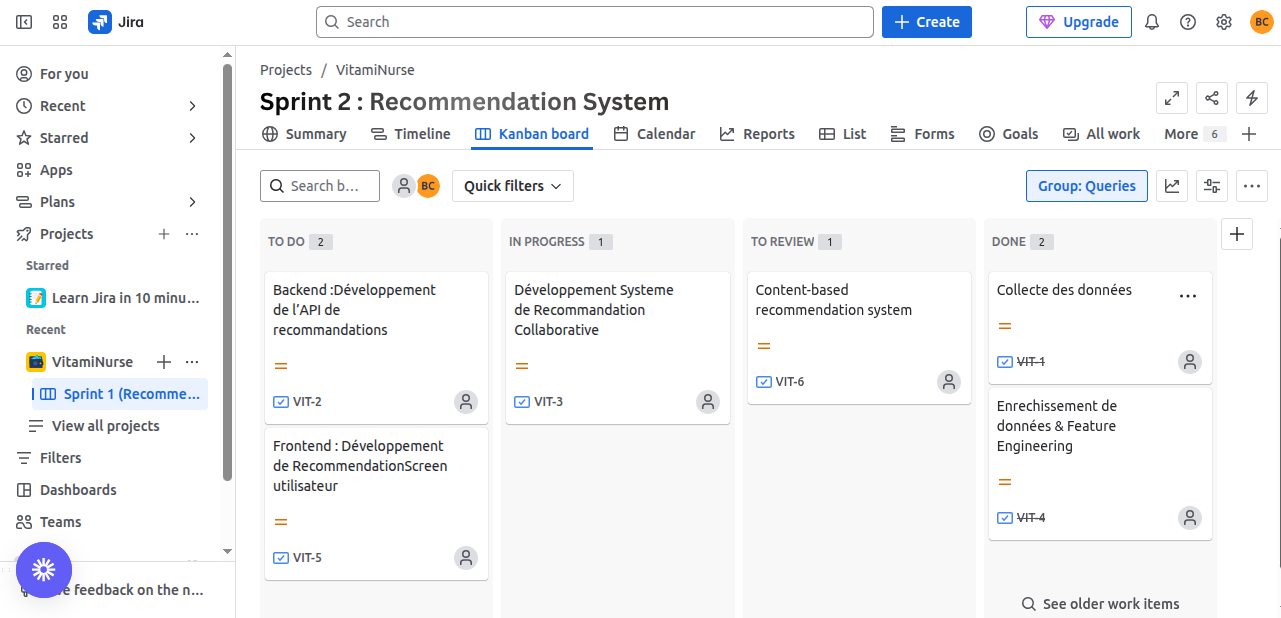
\includegraphics[scale=0.38]{images/kanbanBoard.png}
            \caption{Our Scrumban Board Implementation}
            \label{fig:Tableau_Scrumban}
\end{figure}
\end{center}

The first step in the Scrumban process is to set up the Scrumban board, which is an enhanced version of the Kanban board. It contains all the features, including the product backlog, sprint backlog, and workflow stages (not started, in progress, and under review).

\subsection{Chosen technical methodology}

For the technical execution, we adopted the CRISP-DM for its structured
and iterative approach to solving complex data science problems. It
represents a comprehensive six-phase process includes problem understanding, data exploration, data preparation, modeling, evaluation, and
deployment.
\begin{center}
\begin{figure}[H]
            \centering
            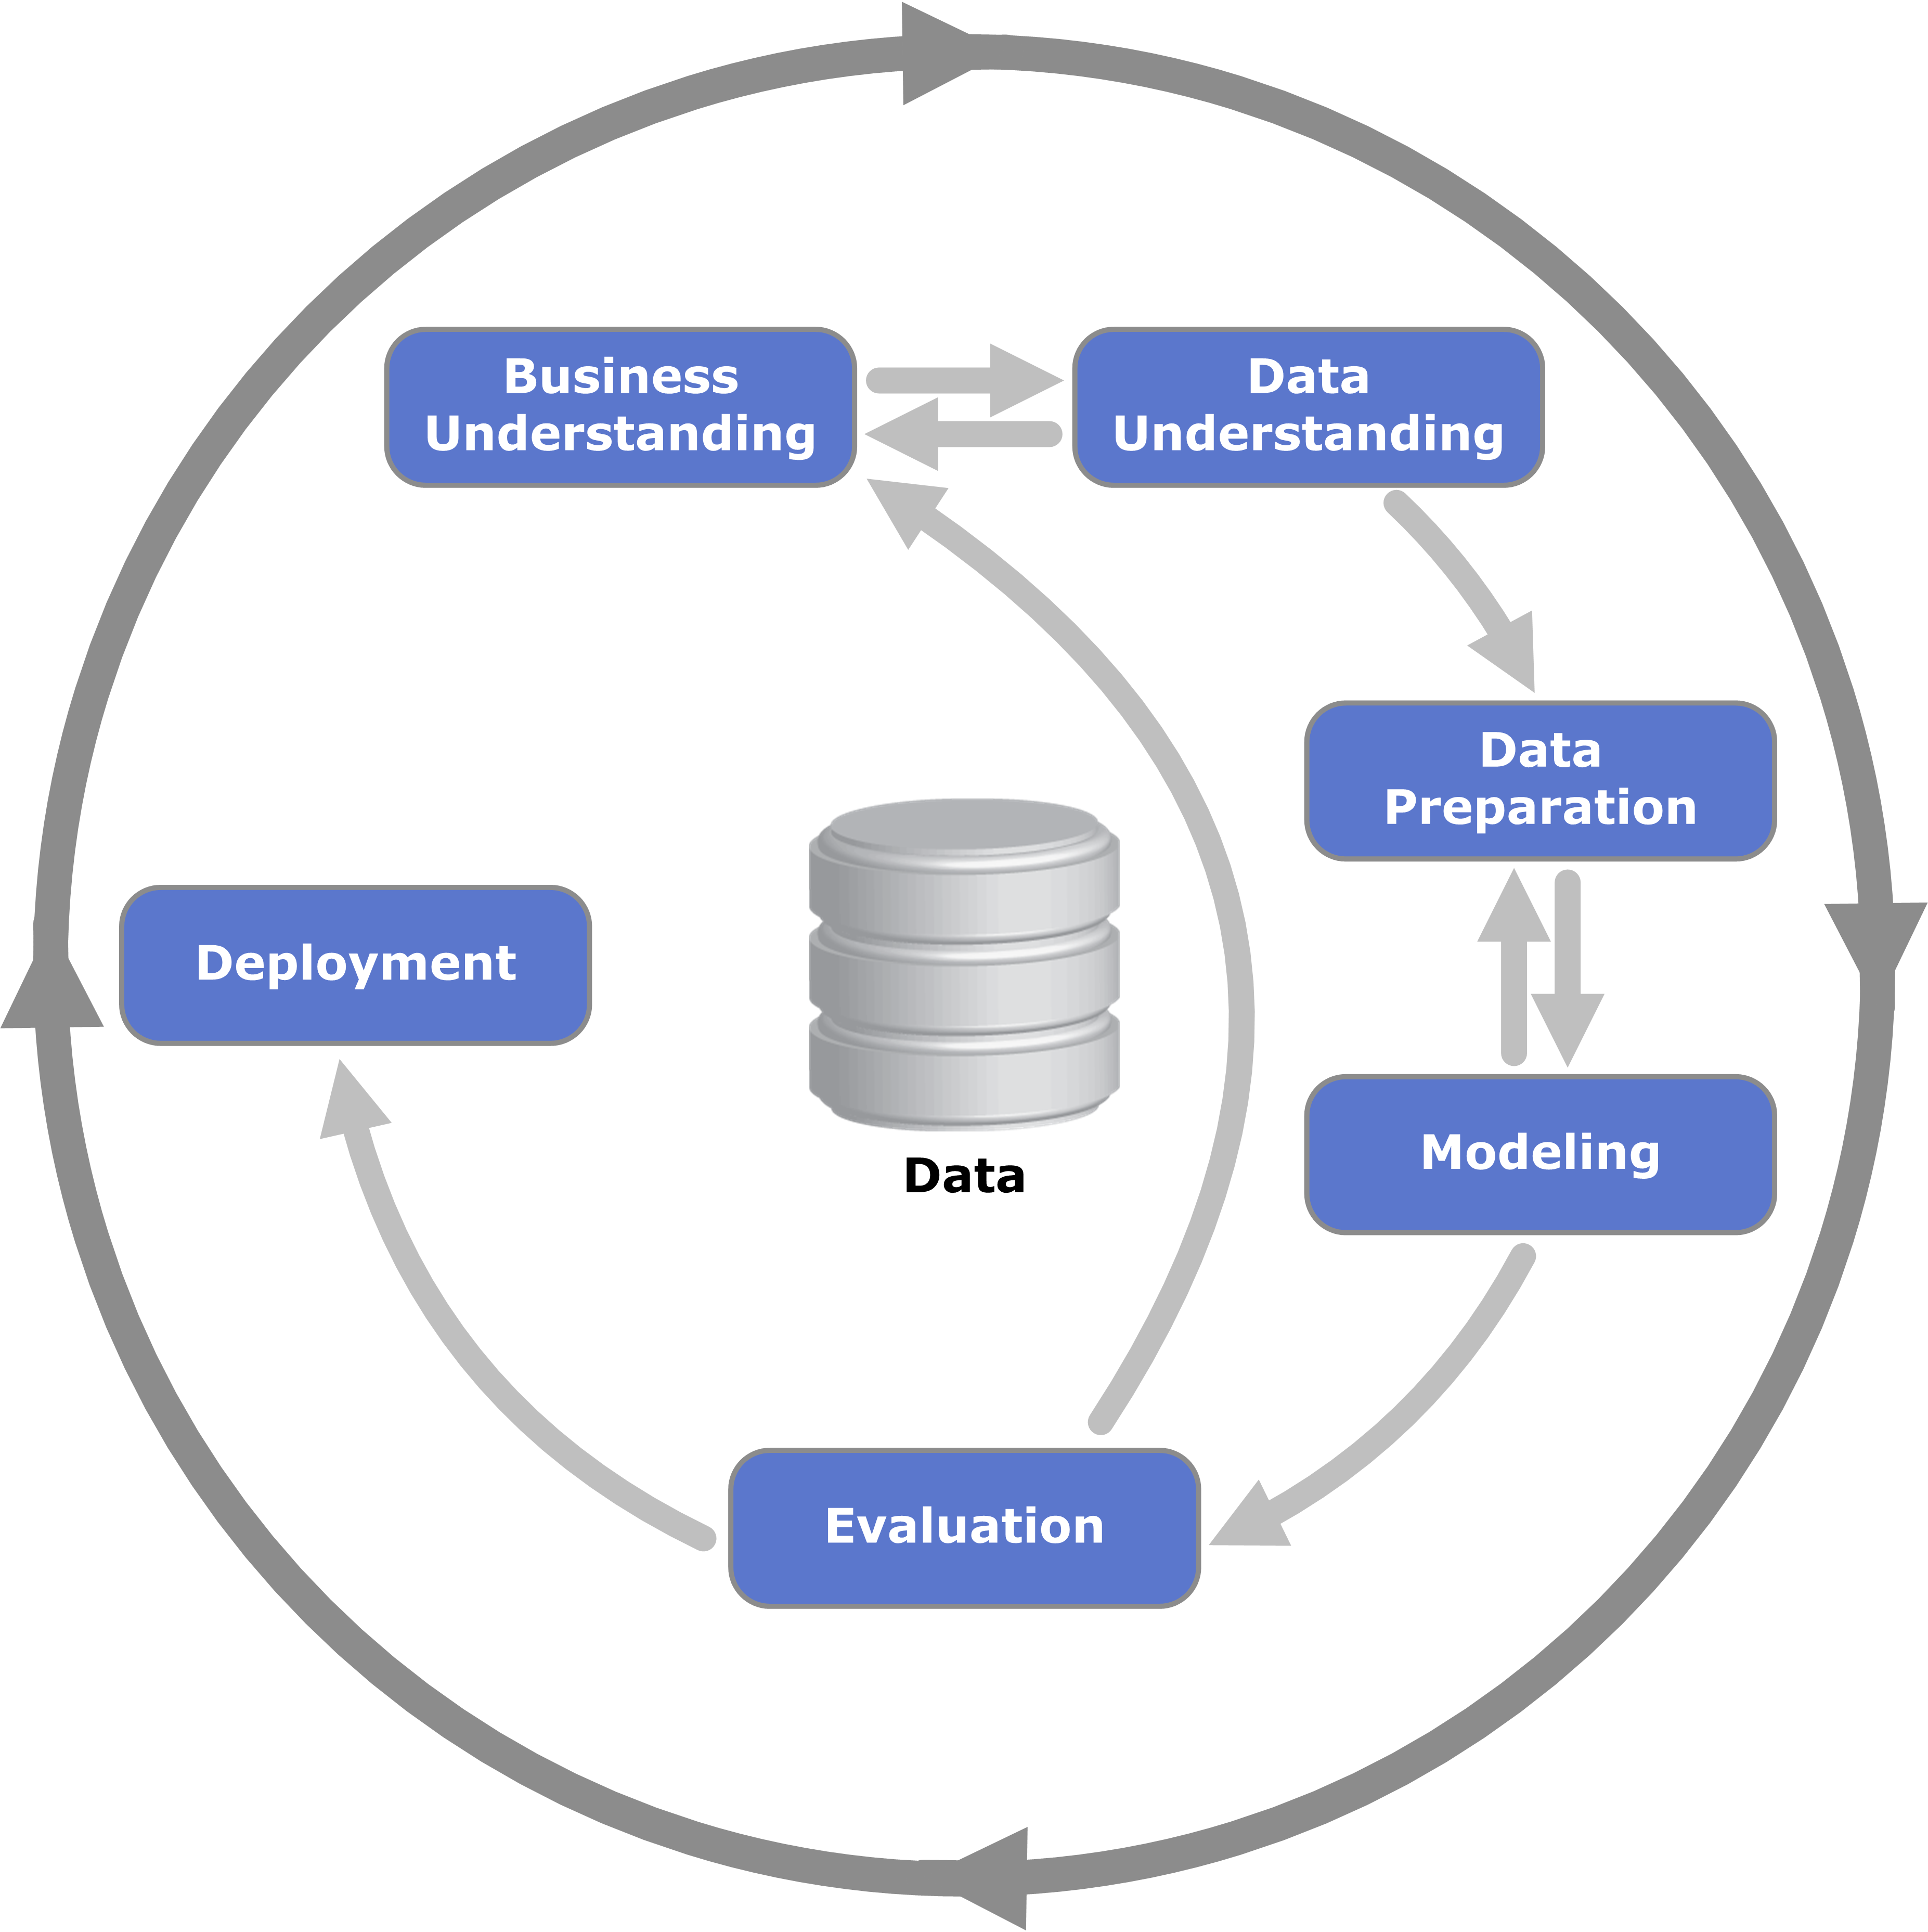
\includegraphics[scale=0.44]{images/CRISP.png}
            \caption{CRISP-DM} 
            \label{fig:CRIS-DM}
        \end{figure}
\end{center}

\par This methodology is particularly well-suited for our project, which involves
developing a personalized recommendation system and an AI assistant
for nutritional guidance. The structured phases of CRISP-DM allow
us to systematically address the challenges of data collection, model development, and deployment while ensuring that we remain aligned
with user needs and project goals.



\section*{Conclusion}
\addcontentsline{toc}{section}{Conclusion}
In this first chapter, we presented the context of our internship project
at ONRTECH, focusing on the development of the VitamiNurse application. We analyzed existing nutritional applications to identify their
strengths and weaknesses, which informed our proposed enhancements
for VitamiNurse. Our solution leverages more artificial intelligence to
improve user nutritional support. The new version of VitamiNurse aims
to provide a more personalized, interactive, and adaptive user experience
through two key features: an advanced recommendation system and a
user-friendly AI assistant.
We also defined the methodologies adopted for the project’s development.
For team organization, the Scrumban method was chosen for its flexibility
and clarity. CRISP-DM was chosen as a technical work methodology, as
it provides a structured approach for data science projects.
This chapter provides a solid foundation for the rest of the work before
moving on to the next chapter, dedicated to the development of the data
pipeline.